\chapter{Current API's\label{currentAPIs}}
\section{Argus}
%https://docs.nvidia.com/jetson/l4t-multimedia/group__LibargusAPI.html

Argus is a camera API that's developed by Nvidia. Argus runs only on Nvidia
hardware, such as the Jetson Orin Nano Developer Kit.

Argus is roughly based on V4L2 though effectively a re-implementation. At the
time Argus was created, V4L2 was still in an early stage. It di not supporting
a variety of features such as multicamera setups etc. hence Argus was created
in order to add the missing features easily. These days V4L2 and Argus are very
close though in later chapters we'll give an overview of what pros and cons
each has.

The reason Argus doesn't use V4L2 is largely a historical one at this point.
At the time Argus was created V4L2 was in an early stage, it had very limited
features. Nvidia created Argus in order to leviate these issues but ended up
with an API that is very similar to V4L2. Automotive for example needed support
for multi camera use cases, this was something that wasn't supported in V4L2 at
the time.

Over time, the API has aged a little though. Today it's still very dependent on
EGL. EGL is a very dated API, like OpenGL it's largely in maintenance mode
today.

\section{libcamera}
libcamera is an open-source C++ embedded camera framework that supports a large
number of complex cameras such as the IMX 219, 477 and many more. It supports
multiple encoders to receive images in for example PNGs/raw images. The primary
target for libcamera is Arm processors in the form of Raspberry PI's, Chrome OS
and Android though many other architectures are also supported\cite{libcameraStack}.
Because image processing algorithms are often proprietary and very secret,
libcamera also allows for binary blobs to be supplied by the vendors. The
vendors do need to submit the "base case" where the camera can take a still
image with decent quality to get the blob approved.

\begin{figure}
    \begin{center}
        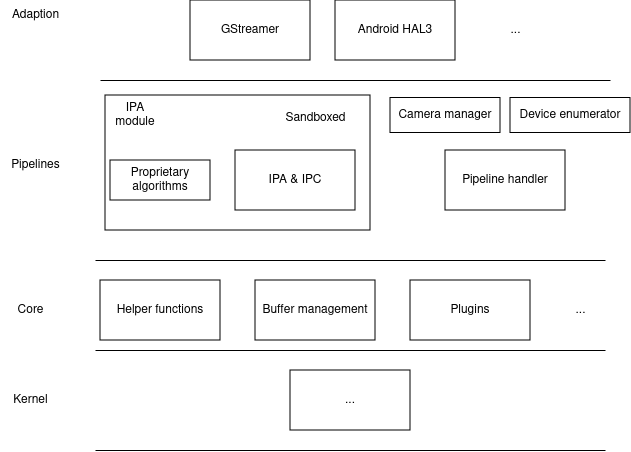
\includegraphics[width=0.60\textwidth]{figures/libcameraarch.png}
    \end{center}
    \caption{High level overview of how the libcamera architecture looks like}
    \label{fig:libcameraarch}
\end{figure}


\section{HAL3}
Hardware Abstraction Layer 3 (HAL3) is the camera API that's included in each
Android phone, it has remarkable features for a mobile phone camera. It was
created to bridge the gap between the higher level the API camera2 and the
lower level hardware API's. It allows for more modification than camera2, while
requiring more work to manage.

% TODO more content

\begin{figure}
    \begin{center}
        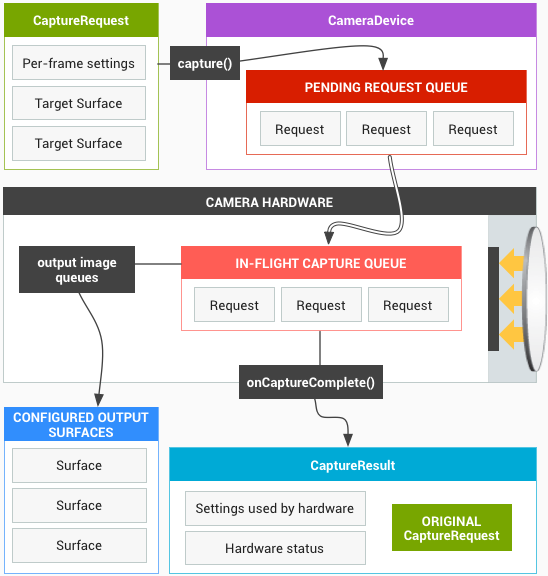
\includegraphics[width=0.5\textwidth]{figures/hal3arch}
    \end{center}
    \caption{HAL3 architecture \cite{hal3arch}}\label{fig:hal3arch}
\end{figure}

\section{Kamaros}
Kamaros is a new API currently (2024) being designed. It's goal is to
standardize the embedded camera frameworks. It's under development, not much can
be mentioned about the API itself due to a spec not being out yet. It hopes to
be easy to use and ability to leverage Vulkan for post processing.
% TODO?

%TODO Gen<I>Cam? it's a much higher level API though might still be worth talking about?
